\subsection{Customer View}

%For the main pages put a mockup and describe it in detail.
The customer view is composed of the pages that are only visible to logged-in clients, therefore no guest can see these.

\begin{center}
    \frame{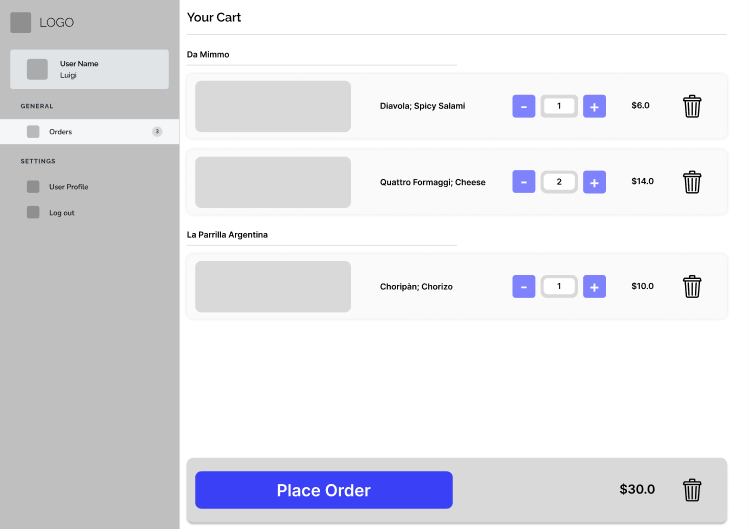
\includegraphics[width=.8\textwidth]{resources/mockup/customer/Cart}}
    \captionof{figure}{Shopping cart page that shows the list of dishes added to the order.}
    \label{fig:customer-Cart}
\end{center}

The virtual shopping cart page, figure \ref{fig:customer-Cart}, shows the current order for the user, listing all the selected dishes grouped by restaurant. The customer can add or subtract to the quantity of a dish, or can just delete it using the trash can button. The interface shows the price of each item and the total bill of the order. The user can complete the order by clicking on the "Place Order" button. Otherwise he can empty his cart by pressing the trash can icon near the bottom.

\begin{center}
    \frame{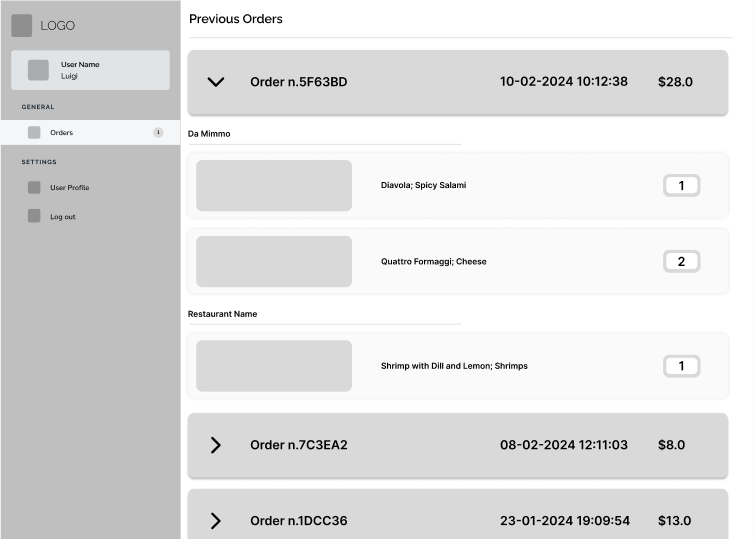
\includegraphics[width=.8\textwidth]{resources/mockup/customer/Previous_orders}}
    \captionof{figure}{Previous orders' page.}
    \label{fig:customer-PreviousOrders}
\end{center}

The previous orders page, figure \ref{fig:customer-PreviousOrders}, shows the identifier, the date and the cost of each of the completed orders. By clicking on the drop down arrow on the left of an order, the customer can see the list of dishes. This page is designed to be scrollable, given that there could be many more completed orders than those that fit the screen.